\documentclass[11.5pt]{article}
\usepackage[utf8]{inputenc}
\usepackage[spanish,activeacute]{babel}
\usepackage{graphicx}
\usepackage{anysize}
\usepackage{subcaption}
\usepackage{tikz}
\usepackage{titlesec}
\setcounter{secnumdepth}{4}
\usepackage{titling}
\usepackage{enumitem}
\usepackage{xcolor}
\usepackage{amsmath}
\usepackage{amssymb}
\usepackage{listings}
\usepackage[most]{tcolorbox}
\usepackage[hidelinks]{hyperref}
\usepackage{array}
\usepackage{tabularx}
\usepackage{tocloft}
\usepackage{textcomp}
\usepackage{fancyhdr}
\usepackage{wrapfig}
\usepackage{fancybox}
\usepackage{float}
\usepackage{booktabs}
\usepackage{longtable}
\usepackage{ragged2e}
\usepackage{colortbl}
\usepackage{xltabular}     % longtable + tabularx (columnas X)

% Colores de estado (acuerdo del curso: verde, amarillo y blanco)
\definecolor{estcompleta}{HTML}{C6EFCE}
\definecolor{estparcial}{HTML}{FFEB9C}
\definecolor{ganttgris}{RGB}{225,225,230}
\definecolor{ganttdiam}{RGB}{210,120,120}
\definecolor{ganttrow}{RGB}{245,245,250}

% Celdas de la Carta Gantt
\newcommand{\gC}{\cellcolor{estcompleta}\rule[-0.35ex]{0pt}{2.6ex}\hspace{0.15em}}
\newcommand{\gP}{\cellcolor{estparcial}\rule[-0.35ex]{0pt}{2.6ex}\hspace{0.15em}}
\newcommand{\gN}{\cellcolor{ganttgris}\rule[-0.35ex]{0pt}{2.6ex}\hspace{0.15em}}
\newcommand{\gdia}{\cellcolor{ganttdiam}\rule[-0.35ex]{0pt}{2.6ex}\hspace{0.15em}\(\blacklozenge\)\hspace{0.15em}}

% Filas por estado
\newcommand{\filaC}{\rowcolor{estcompleta}}
\newcommand{\filaP}{\rowcolor{estparcial}}

\definecolor{codecomment}{rgb}{0.13,0.55,0.13}
\definecolor{codegray}{rgb}{0.5,0.5,0.5}
\definecolor{codepurple}{rgb}{0.58,0,0.82}
\definecolor{backcolour}{rgb}{0.95,0.95,0.92}

\lstdefinestyle{mystyle}{
    backgroundcolor=\color{backcolour},
    commentstyle=\color{codecomment},
    stringstyle=\color{codepurple},
    basicstyle=\footnotesize\ttfamily,
    breakatwhitespace=false,
    breaklines=true,
    captionpos=b,
    keepspaces=true,
    showspaces=false,
    showstringspaces=false,
    showtabs=false,
    tabsize=3
}
\lstset{style=mystyle}

%%%%%%%%%%%%%%%%%%%%%%%%%%%%%%%%%%%%%%%%%%%%%%%%%%%%%%%%%%%%%%%%%%%%%%%%%%%%%

\titleformat{\paragraph}
{\normalfont\normalsize\bfseries}{\theparagraph}{1em}{}
\titlespacing*{\paragraph}
{0pt}{3.25ex plus 1ex minus .2ex}{1.5ex plus .2ex}

\marginsize{1.5cm}{1.5cm}{1cm}{1cm}
\graphicspath{ {imagenes/} {../../evidencias/reportes/} }

% --- Estilo para tablas anchas ---
\newcolumntype{L}[1]{>{\RaggedRight\arraybackslash}p{#1}}
\newcolumntype{C}[1]{>{\Centering\arraybackslash}p{#1}}

\begin{document}

% ==========================================================
% PORTADA
% ==========================================================
\pagestyle{plain}{
\pagestyle{empty}
\noindent

{\small
\begin{tabular}{p{0.40\textwidth} p{0.50\textwidth}}

\includegraphics[scale=0.1]{usm.jpg} &

\includegraphics[scale=0.4]{elo.jpg}
\end{tabular}
}

\begin{center}

\rule{\linewidth}{0.5mm}\\[0.4cm]
\par\vspace{0.25cm}
\Huge\textbf{Detección y localización de patologías torácicas en radiografías mediante Deep Learning}\\[0.15cm]
\Large\textbf{Documento de Avance de la Solución --- Hito 2}

\par\vspace{0.5cm}
\rule{\linewidth}{0.5mm}\\[4.0cm]

\vspace{1.5cm}
\date{6 de noviembre de 2026}
\Large{
\begin{tabular}{rl}
\textbf{Fecha}       &  \thedate \\
\textbf{\begin{tabular}[c]{@{}l@{}}Integrantes: \\ $\;$ \\ $\;$ \\ $\;$ \end{tabular}} & \begin{tabular}[c]{@{}l@{}} Benjamin Esteban Arias Vega \\ Karime Andrea Jarufe Escobar \\ Nicolas Eduardo Severino Palma \\ Hans David Varela Antilao \end{tabular} \\
\textbf{Asignatura:}  & TEL328 \\
\textbf{Profesor:}  & Marcos Zúñiga \\
\textbf{Versión:} & 2.0 (Hito 2) \\
\end{tabular}
}
\end{center}
\clearpage
}

\pagestyle{fancyplain}
\fancyhf{}
\lhead{ \fancyplain{}{TEL328}}
\rhead{ \fancyplain{}{2026} }
\lfoot{ \fancyplain{}{USM 2026 - 2} }
\rfoot{ \fancyplain{}{\thepage} }
\renewcommand{\footrulewidth}{0.5pt}
%%%%%%%%%%%%%%%%%%%%%%%%%%%%%%%%%%%%%%%%%%%%%%%%%%%%%%%%%%%%%%%%%%%%

\begin{center}
\tableofcontents
\end{center}

\begin{center}
\listoffigures
\end{center}

\begin{center}
\listoftables
\end{center}

\clearpage
\newpage

% ==========================================================
\section{Introducción}
% ==========================================================

El proyecto desarrolla un sistema que recibe una radiografía de tórax en formato DICOM, la procesa con un modelo de Deep Learning y entrega las patologías probables y su ubicación aproximada sobre la imagen. El modelo se entrena con el dataset público \textbf{NIH ChestX-ray14} [1], que contiene 112.120 radiografías frontales de 30.805 pacientes, con etiquetas para 14 patologías.

El sistema es una \textbf{herramienta de apoyo y prototipo académico}, no un dispositivo de diagnóstico: cualquier resultado debe ser revisado por un profesional de la salud.

Este documento corresponde al Hito 2 (corte: semana 14, del 02/11 al 06/11) y continúa el Documento de Análisis y Diseño del Hito 1, al que se remite para el diagnóstico del problema, el estado del arte, los perfiles de usuario y el diseño original. Aquí se describe lo implementado, los resultados obtenidos, las pruebas ejecutadas y el trabajo pendiente. Las evidencias citadas están en la carpeta \texttt{evidencias/} de la rama \texttt{hito-2} del repositorio del proyecto, y su índice se encuentra en el Anexo~\ref{sec:evidencias}.

\subsection{Resumen del avance}

\begin{itemize}
    \item \textbf{Implementado:} verificación del dataset, división por paciente, estadísticas, pesos por clase, subconjunto de prueba, script de entrenamiento y aplicación con lector DICOM, inferencia, Grad-CAM, cajas delimitadoras y exportación.
    \item \textbf{Resultado del modelo:} solo existe un modelo de prueba, entrenado con 2.000 imágenes durante 2 épocas, con AUC de validación de 0,61. Sirve para comprobar que el flujo funciona, no como medida de desempeño final.
    \item \textbf{Pruebas:} 26 de 26 pruebas automatizadas aprobadas, sin depender del modelo entrenado.
    \item \textbf{Pendiente:} entrenamiento completo con las 76.277 imágenes de entrenamiento, evaluación AUC-ROC en el conjunto de prueba, evaluación IoU de las cajas y pruebas de sistema y usabilidad.
\end{itemize}

% ==========================================================
\section{Planificación del Proyecto}
% ==========================================================

La planificación sigue la estructura presentada en el material del curso \textit{Elementos Iniciales de Planificación de Proyectos}: objetivo general, objetivos específicos, actividades, tareas con un entregable asociado y milestones. Los estados y porcentajes provienen de la Bitácora 2.

\subsection{Objetivo General (Goal)}

Desarrollar un sistema de apoyo al análisis de radiografías de tórax, basado en Deep Learning, que detecte patologías pulmonares y su ubicación a partir de una imagen DICOM, utilizando el dataset NIH ChestX-ray14.

\subsection{Objetivos Específicos}

Cada objetivo parte con un verbo de acción y se detalla según las partes propuestas en el material del curso. La población afectada es el equipo de desarrollo en O1 y O5, y los perfiles de usuario definidos en el Hito 1 en O2, O3 y O4.

\begin{table}[H]
\centering
\footnotesize
\caption{Objetivos específicos y criterios de éxito}
\label{tab:objetivos}
\begin{tabularx}{\textwidth}{L{4.5cm} L{1.1cm} X X L{1.1cm}}
\toprule
Objetivo (qué) & Cuándo & Cómo y criterio & Nivel de éxito & Avance \\
\midrule
\textbf{O1.} Analizar y preparar el dataset NIH ChestX-ray14 con división por paciente & S12 & Scripts de verificación, división y estadísticas; evidencia en logs y reportes & Conteos oficiales coinciden y 0 pacientes en común entre conjuntos (PM1) & 100\% \\
\textbf{O2.} Entrenar y evaluar un clasificador multi-etiqueta de 14 patologías & S16 & DenseNet-121 con transferencia de aprendizaje; AUC-ROC por patología en el conjunto de prueba & AUC-ROC reportado para las 14 patologías y promedio cercano a la literatura (PM2). Meta numérica por fijar tras el entrenamiento completo (RNF8) & 67\% \\
\textbf{O3.} Implementar y evaluar la localización de regiones afectadas & S16 & Grad-CAM y conversión a cajas; comparación con las 984 cajas reales & IoU y proporción de aciertos reportados a distintos umbrales (PM3) & 67\% \\
\textbf{O4.} Desarrollar una aplicación que reciba DICOM y muestre patologías y ubicación & S17 & Aplicación local con los módulos integrados; pruebas de sistema & Resultado en menos de 10 s (RNF1) y en no más de 3 pasos (RNF2) & 100\% \\
\textbf{O5.} Diseñar y ejecutar el plan de pruebas & S18 & Pruebas de modelo, unitarias, de sistema y de usabilidad & Todas las pruebas PM, PU y PS ejecutadas e informadas & 67\% \\
\bottomrule
\end{tabularx}
\end{table}

El avance de O4 corresponde a la implementación e integración registradas en la Bitácora 2. Sus niveles de éxito se medirán con las pruebas PS1 y PS5, que siguen pendientes (sección~\ref{sec:pruebas}).

\subsection{Actividades y Milestones}

\textit{Semanas y fechas según el calendario del curso. La participación corresponde a la propuesta del Hito 1.}

\begin{xltabular}{\textwidth}{X L{2.4cm} L{2.1cm} L{2cm} L{2cm} L{1.3cm}}
\caption{Actividades y milestones}
\label{tab:actividades}\\
\toprule
Elemento & Responsable & Participación equipo & Fecha comienzo & Fecha término & \% avance \\
\midrule
\endfirsthead

\toprule
Elemento & Responsable & Participación equipo & Fecha comienzo & Fecha término & \% avance \\
\midrule
\endhead

\midrule
\multicolumn{6}{r}{\footnotesize\textit{Continúa en la página siguiente\ldots}}\\
\endfoot

\bottomrule
\endlastfoot

\filaC \textbf{A1.1} Análisis del dataset (O1) & Nicolas Severino & 25\% c/u & 21/09 (S8) & 02/10 (S9) & 100\% \\
\filaC \textbf{A1.2} Pipeline de datos (O1) & Benjamin Arias & 25\% c/u & 12/10 (S11) & 23/10 (S12) & 100\% \\
\filaP \textbf{A2.1} Modelo base (O2) & Hans Varela & 25\% c/u & 12/10 (S11) & 06/11 (S14) & 83\% \\
\filaP \textbf{A2.2} Ajuste y evaluación (O2) & Hans Varela & 25\% c/u & 02/11 (S14) & 20/11 (S16) & 50\% \\
\filaP \textbf{A3.1} Localización con Grad-CAM (O3) & Karime Jarufe & 25\% c/u & 02/11 (S14) & 20/11 (S16) & 67\% \\
\filaC \textbf{A4.1} Lectura y preprocesamiento de DICOM (O4) & Benjamin Arias & 25\% c/u & 12/10 (S11) & 30/10 (S13) & 100\% \\
\filaC \textbf{A4.2} Interfaz gráfica (O4) & Karime Jarufe & 25\% c/u & 28/09 (S9) & 27/11 (S17) & 100\% \\
\filaC \textbf{A5.1} Diseño de pruebas (O5) & Nicolas Severino & 25\% c/u & 28/09 (S9) & 09/10 (S10) & 100\% \\
\filaP \textbf{A5.2} Ejecución de pruebas (O5) & Nicolas Severino & 25\% c/u & 02/11 (S14) & 04/12 (S18) & 33\% \\
\filaP \textbf{G1.1} Documentación, seguimiento y presentaciones & Todo el equipo & 25\% c/u & 21/09 (S8) & 04/12 (S18) & 71\% \\
\filaC \textbf{G1.2} Definición y delimitación del problema & Todo el equipo & 25\% c/u & 21/09 (S8) & 02/10 (S9) & 100\% \\
\filaC \textbf{Milestone 1:} Análisis y Diseño (documento, presentación y Bitácora 1) & Todo el equipo & 25\% c/u & 21/09 (S8) & 09/10 (S10) & 100\% \\
\filaC \textbf{Milestone 2 (Bitácora 2):} avance con modelo base y lector DICOM & Todo el equipo & 25\% c/u & 12/10 (S11) & 06/11 (S14) & 100\% \\
\filaP \textbf{Milestone 3:} sistema integrado con localización e interfaz & Todo el equipo & 25\% c/u & 02/11 (S14) & 27/11 (S17) & 60\% \\
\textbf{Milestone 4:} presentación en la Feria y evaluación final (Bitácora 3) & Todo el equipo & 25\% c/u & 23/11 (S17) & 04/12 (S18) & 0\% \\
\end{xltabular}

El Milestone 2 se considera entregado con un modelo base de prueba y el lector DICOM. El entrenamiento completo sigue pendiente en la tarea T2.1.3.

\subsection{Tareas y entregables}

Según el material del curso, una tarea es válida solo si tiene un entregable asociado. Se usa el acuerdo de colores del curso: \colorbox{estcompleta}{verde} para completada, \colorbox{estparcial}{amarillo} para asignada en el período o parcialmente lograda, y blanco para no asignada.

{\footnotesize
\begin{xltabular}{\textwidth}{L{1.15cm} X L{2.5cm} L{4.2cm} L{0.95cm}}
\caption{Tareas, autores y entregables}
\label{tab:tareas}\\
\toprule
ID & Tarea & Autor(es) & Entregable & Avance \\
\midrule
\endfirsthead

\toprule
ID & Tarea & Autor(es) & Entregable & Avance \\
\midrule
\endhead

\midrule
\multicolumn{5}{r}{\textit{Continúa en la página siguiente\ldots}}\\
\endfoot

\bottomrule
\endlastfoot

\filaC T1.1.1 & Descargar el dataset y revisar su estructura y metadatos & Hans Varela & Dataset local e inventario de archivos & 100\% \\
\filaC T1.1.2 & Estadísticas de clases y matriz de co-ocurrencia & Hans Varela & Script, reporte y gráficos de distribución & 100\% \\
\filaC T1.2.1 & División por paciente y validación interna & Benjamin Arias & Script de división de datos & 100\% \\
\filaC T1.2.2 & Preprocesamiento (PRE) y aumento de datos & Benjamin Arias & Módulo PRE (código) & 100\% \\
\filaC T2.1.1 & Configurar TensorFlow/Keras y GPU de entrenamiento & Nicolas Severino & Guía de entorno y dependencias & 100\% \\
\filaC T2.1.2 & Clasificador DenseNet-121 con transferencia de aprendizaje & Nicolas Severino & Script del modelo (módulo CLS) & 100\% \\
\filaP T2.1.3 & Primer entrenamiento y curvas de aprendizaje & Nicolas Severino & Pesos del modelo y gráficos de pérdida & 50\% \\
\filaC T2.2.1 & Ponderación de clases y ajuste de hiperparámetros & Nicolas Severino & Registro de experimentos & 100\% \\
T2.2.2 & Evaluación AUC-ROC por patología en el conjunto de prueba & --- & Informe de métricas & 0\% \\
\filaC T3.1.1 & Implementar Grad-CAM sobre el clasificador & Karime Jarufe & Módulo LOC (código) & 100\% \\
\filaC T3.1.2 & Conversión de mapas de calor a cajas delimitadoras & Karime Jarufe & Función \texttt{to\_boxes} y ejemplos visuales & 100\% \\
T3.1.3 & Evaluación de IoU con \texttt{BBox\_List\_2017} & Karime Jarufe & Informe de IoU & 0\% \\
\filaC T4.1.1 & Lector DICOM con validación (DCM) & Benjamin Arias & Módulo DCM (código) & 100\% \\
\filaC T4.1.2 & Pruebas de consistencia entre DICOM y PNG & Benjamin Arias & Informe de consistencia & 100\% \\
\filaC T4.2.1 & Diseño de mockups de interfaces (Hito 1) & Karime Jarufe & Prototipos y tabla de eventos & 100\% \\
\filaC T4.2.2 & Implementar la GUI según los mockups & Karime Jarufe & Aplicación GUI (código) & 100\% \\
\filaC T4.2.3 & Integrar GUI con DCM, PRE, CLS y LOC & Karime Jarufe, Benjamin Arias & Sistema integrado & 100\% \\
\filaC T5.1.1 & Diseñar el plan de pruebas & Nicolas Severino & Plan de pruebas (Documento del Hito 1) & 100\% \\
\filaC T5.2.1 & Ejecutar pruebas unitarias de módulos & Hans Varela & Scripts de prueba y resultados & 100\% \\
T5.2.2 & Ejecutar pruebas de sistema y de usabilidad & Todo el equipo & Informe de pruebas & 0\% \\
T5.2.3 & Informe final y conclusiones & Todo el equipo & Informe final & 0\% \\
\filaC G1.1.1 & Documento de Análisis y Diseño v1.0 & Todo el equipo & Documento & 100\% \\
\filaC G1.1.2 & Presentación de Análisis y Diseño & Todo el equipo & Presentación & 100\% \\
\filaC G1.1.3 & Bitácora 1 & Todo el equipo & Planilla de bitácora & 100\% \\
\filaP G1.1.4 & Reuniones semanales de seguimiento (ciclo scrum) & Todo el equipo & Actas breves de reunión & En curso \\
\filaC G1.1.5 & Bitácora 2 & Todo el equipo & Planilla de bitácora y avance & 100\% \\
G1.1.6 & Presentación y material para la Feria & --- & Presentación o póster & 0\% \\
G1.1.7 & Bitácora 3 & --- & Planilla de bitácora e informe final & 0\% \\
\filaC G1.2.1 & Definir el problema, su alcance y sus límites & Todo el equipo & Documento del Hito 1 & 100\% \\
\end{xltabular}
}

\subsection{Carta Gantt}

Planificación por semana del calendario del curso, con el color del estado de cada actividad en el corte de la semana 14.
\colorbox{estcompleta}{\rule{0pt}{1.4ex}\hspace{1.2ex}} = completada;
\colorbox{estparcial}{\rule{0pt}{1.4ex}\hspace{1.2ex}} = parcial o asignada;
\colorbox{ganttgris}{\rule{0pt}{1.4ex}\hspace{1.2ex}} = planificada sin iniciar;
\textcolor{ganttdiam}{\(\blacklozenge\)} = entrega del curso.

\begin{table}[H]
\centering
\footnotesize
\caption{Carta Gantt}
\label{tab:gantt}
\setlength{\tabcolsep}{2pt}
\renewcommand{\arraystretch}{1.35}
\resizebox{\textwidth}{!}{%
\begin{tabular}{l *{11}{c}}
\toprule
\rowcolor{ganttrow}
Actividad & S8 21/09 & S9 28/09 & S10 05/10 & S11 12/10 & S12 19/10 & S13 26/10 & S14 02/11 & S15 09/11 & S16 16/11 & S17 23/11 & S18 30/11 \\
\midrule
A1.1 Análisis del dataset    & \gC & \gC &     &     &     &     &     &     &     &     &     \\
A1.2 Pipeline de datos       &     &     &     & \gC & \gC &     &     &     &     &     &     \\
A2.1 Modelo base             &     &     &     & \gP & \gP & \gP & \gP &     &     &     &     \\
A2.2 Ajuste y evaluación     &     &     &     &     &     &     & \gP & \gP & \gP &     &     \\
A3.1 Localización (Grad-CAM) &     &     &     &     &     &     & \gP & \gP & \gP &     &     \\
A4.1 Lectura de DICOM        &     &     &     & \gC & \gC & \gC &     &     &     &     &     \\
A4.2 Interfaz gráfica        &     & \gC & \gC & \gC & \gC & \gC & \gC & \gC & \gC & \gC &     \\
A5.1 Diseño de pruebas       &     & \gC & \gC &     &     &     &     &     &     &     &     \\
A5.2 Ejecución de pruebas    &     &     &     &     &     &     & \gP & \gP & \gP & \gP & \gP \\
G1.1 Gestión y seguimiento   & \gP & \gP & \gP & \gP & \gP & \gP & \gP & \gP & \gP & \gP & \gP \\
G1.2 Definición del problema & \gC & \gC &     &     &     &     &     &     &     &     &     \\
Milestone 1                  & \gC & \gC & \gC &     &     &     &     &     &     &     &     \\
Milestone 2 (Bitácora 2)     &     &     &     & \gC & \gC & \gC & \gC &     &     &     &     \\
Milestone 3                  &     &     &     &     &     &     & \gP & \gP & \gP & \gP &     \\
Milestone 4                  &     &     &     &     &     &     &     &     &     & \gN & \gN \\
Entregas del curso           &     &     & \gdia &   &     &     & \gdia &   &     &     & \gdia \\
\bottomrule
\end{tabular}%
}
\end{table}

\subsection{Nivel de madurez tecnológica}

Usando la escala TRL del material del curso, el equipo estima el prototipo entre \textbf{TRL 3} (prueba de concepto de funciones críticas) y \textbf{TRL 4} (validación de componentes en laboratorio). La cadena completa funciona con un modelo de prueba. Para sostener TRL 4 falta validar el modelo completo con las pruebas PM2 y PM3.

% ==========================================================
\section{Solución desarrollada}
% ==========================================================

\subsection{Scripts del proyecto}

La solución se organizó como una secuencia de scripts numerados en \texttt{evidencias/codigo/}. Cada uno usa como entrada la salida de los anteriores.

\begin{table}[H]
\centering
\footnotesize
\caption{Scripts de la solución}
\label{tab:scripts}
\begin{tabularx}{\textwidth}{L{3.9cm} X L{4.3cm}}
\toprule
Script & Función & Salida principal \\
\midrule
\texttt{01\_verificar\_dataset.py} & Cuenta imágenes, pacientes y etiquetas, y los compara con los valores esperados del dataset & Reporte en consola \\
\texttt{02\_split\_dataset.py} & Divide en entrenamiento, validación y prueba, sin repetir pacientes entre conjuntos & \texttt{train.csv}, \texttt{val.csv}, \texttt{test.csv} \\
\texttt{02-1\_analisis\_dataset.py} & Calcula estadísticas de clases, hallazgos por imagen y co-ocurrencia & \texttt{estadisticas.md} y gráficos \\
\texttt{03\_calcular\_pesos.py} & Calcula los pesos por clase para compensar el desbalance & \texttt{class\_weights.json} \\
\texttt{04\_crear\_subconjunto.py} & Crea un subconjunto de 2.000 imágenes de entrenamiento y 500 de validación para pruebas rápidas & \texttt{debug\_train.csv}, \texttt{debug\_val.csv} \\
\texttt{05\_entrenar.py} & Entrena el modelo; la opción \texttt{-{}-debug} elige el subconjunto y, sin ella, usa el conjunto completo & \texttt{modelo\_base.keras} y registros por etapa \\
\texttt{06\_gui.py} & Aplicación gráfica: lectura DICOM, inferencia, Grad-CAM, cajas y exportación & Archivos en \texttt{resultados/} \\
\texttt{11\_reporte\_test.py} & Ejecuta las pruebas automatizadas y genera su reporte & \texttt{tests\_sin\_modelo.md} \\
\bottomrule
\end{tabularx}
\end{table}

\subsection{Preparación de datos}

\paragraph{Verificación (01).} Compara el total de filas y los conteos de las 14 patologías y de ``No Finding'' con los valores esperados. Termina con código de error si encuentra diferencias.

\paragraph{División por paciente (02).} Usa las listas oficiales \texttt{train\_val\_list.txt} y \texttt{test\_list.txt}. Dentro de \texttt{train\_val} separa el 12\% de los pacientes para validación con \texttt{GroupShuffleSplit} y semilla 42, y detiene la ejecución si un paciente aparece en más de un conjunto.

\paragraph{Pesos por clase (03).} Para cada patología calcula $w = \sqrt{(N-P)/P}$, donde $N$ es el total de imágenes de entrenamiento y $P$ las positivas. La raíz suaviza la diferencia entre clases: la razón entre el peso mayor y el menor baja de 126 a 11 veces.

\paragraph{Subconjunto de prueba (04).} Selecciona primero hasta 60 positivos por patología, partiendo por las más raras, y completa con imágenes al azar hasta llegar a 2.000. Permite comprobar el flujo de entrenamiento sin esperar un entrenamiento completo.

\subsection{Modelo y entrenamiento}

\begin{itemize}
    \item \textbf{Arquitectura:} DenseNet-121 [4] preentrenada en ImageNet, seguida de \textit{Global Average Pooling}, \textit{Dropout} de 0,3 y una capa densa de 14 salidas con activación sigmoide. Tiene 7.051.854 parámetros en total.
    \item \textbf{Preprocesamiento:} imagen en escala de grises redimensionada a 224$\times$224, replicada en 3 canales y normalizada con la función de DenseNet.
    \item \textbf{Aumento de datos:} rotación de $\pm$10$^\circ$, zoom de $\pm$10\% y variaciones leves de brillo y contraste. No se usa volteo horizontal, porque cambia el lado del corazón.
    \item \textbf{Pérdida:} entropía cruzada binaria con el peso del Cuadro~\ref{tab:pesos} en el término positivo.
    \item \textbf{Etapa 1:} red base congelada, 3 épocas por defecto y tasa de aprendizaje de $10^{-3}$.
    \item \textbf{Etapa 2:} ajuste fino de las últimas 60 capas, 10 épocas por defecto y tasa de $10^{-5}$. Las capas \textit{BatchNormalization} permanecen congeladas.
    \item \textbf{Control:} guarda el mejor modelo según el AUC de validación, con detención temprana y reducción de la tasa de aprendizaje.
\end{itemize}

\subsection{Localización}

Para cada patología, \texttt{06\_gui.py} aplica Grad-CAM [3] sobre la capa \texttt{relu}, la última activación convolucional de la red. El mapa se binariza en 0,5 y se buscan componentes conexas con OpenCV. Se descartan las que ocupan menos del 0,5\% de la imagen y se conservan hasta dos por patología, convertidas en cajas a la escala de la imagen original.

\subsection{Ambiente de desarrollo}

\begin{itemize}
    \item \textbf{Hardware de entrenamiento:} GPU AMD Radeon RX 9070 XT (16 GB de VRAM) con ROCm.
    \item \textbf{Software:} Linux, Python 3.12.16, TensorFlow 2.21 (compilación propia) con precisión mixta, \texttt{pydicom}, OpenCV, Pillow, Pandas, scikit-learn, Gradio y pytest.
    \item \textbf{Dataset:} NIH ChestX-ray14, que no se incluye en el repositorio.
\end{itemize}

% ==========================================================
\section{Resultados}
% ==========================================================

\subsection{Verificación y estadísticas del dataset}

El script 01 confirmó las 112.120 imágenes y los 30.805 pacientes, y los 15 conteos coincidieron con los valores esperados. El 53,84\% de las imágenes no tiene hallazgos y el 18,55\% tiene dos o más patologías.

\begin{figure}[H]
    \centering
    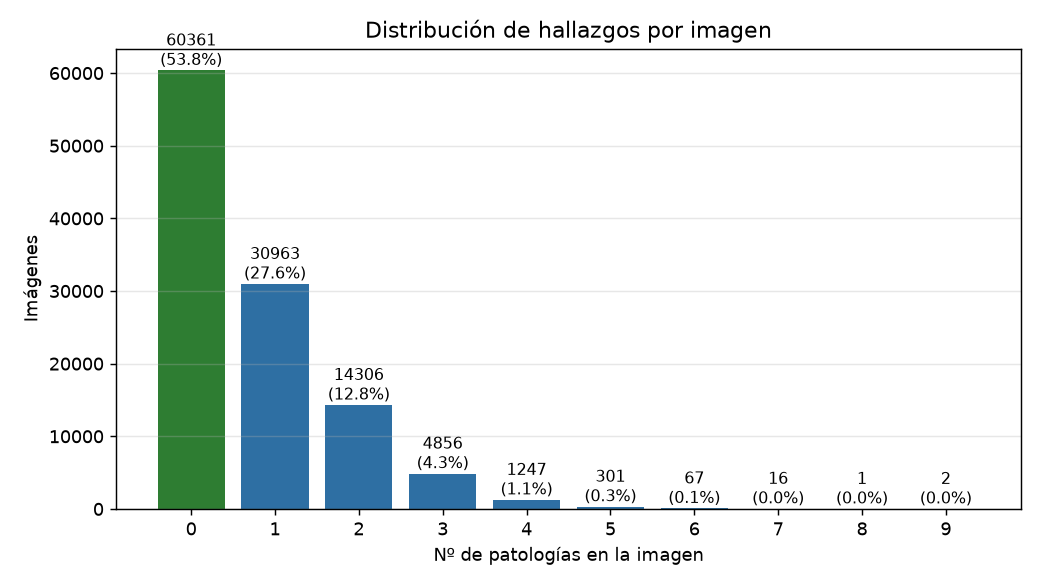
\includegraphics[width=0.46\linewidth]{distribucion.png}
    \caption{Número de hallazgos por imagen}
    \label{fig:distribucion}
\end{figure}

La co-ocurrencia se midió con el \textit{lift}, es decir, la razón entre la frecuencia conjunta observada y la esperada por azar. Un valor mayor que 1 indica que dos patologías aparecen juntas más de lo esperado.

\begin{figure}[H]
    \centering
    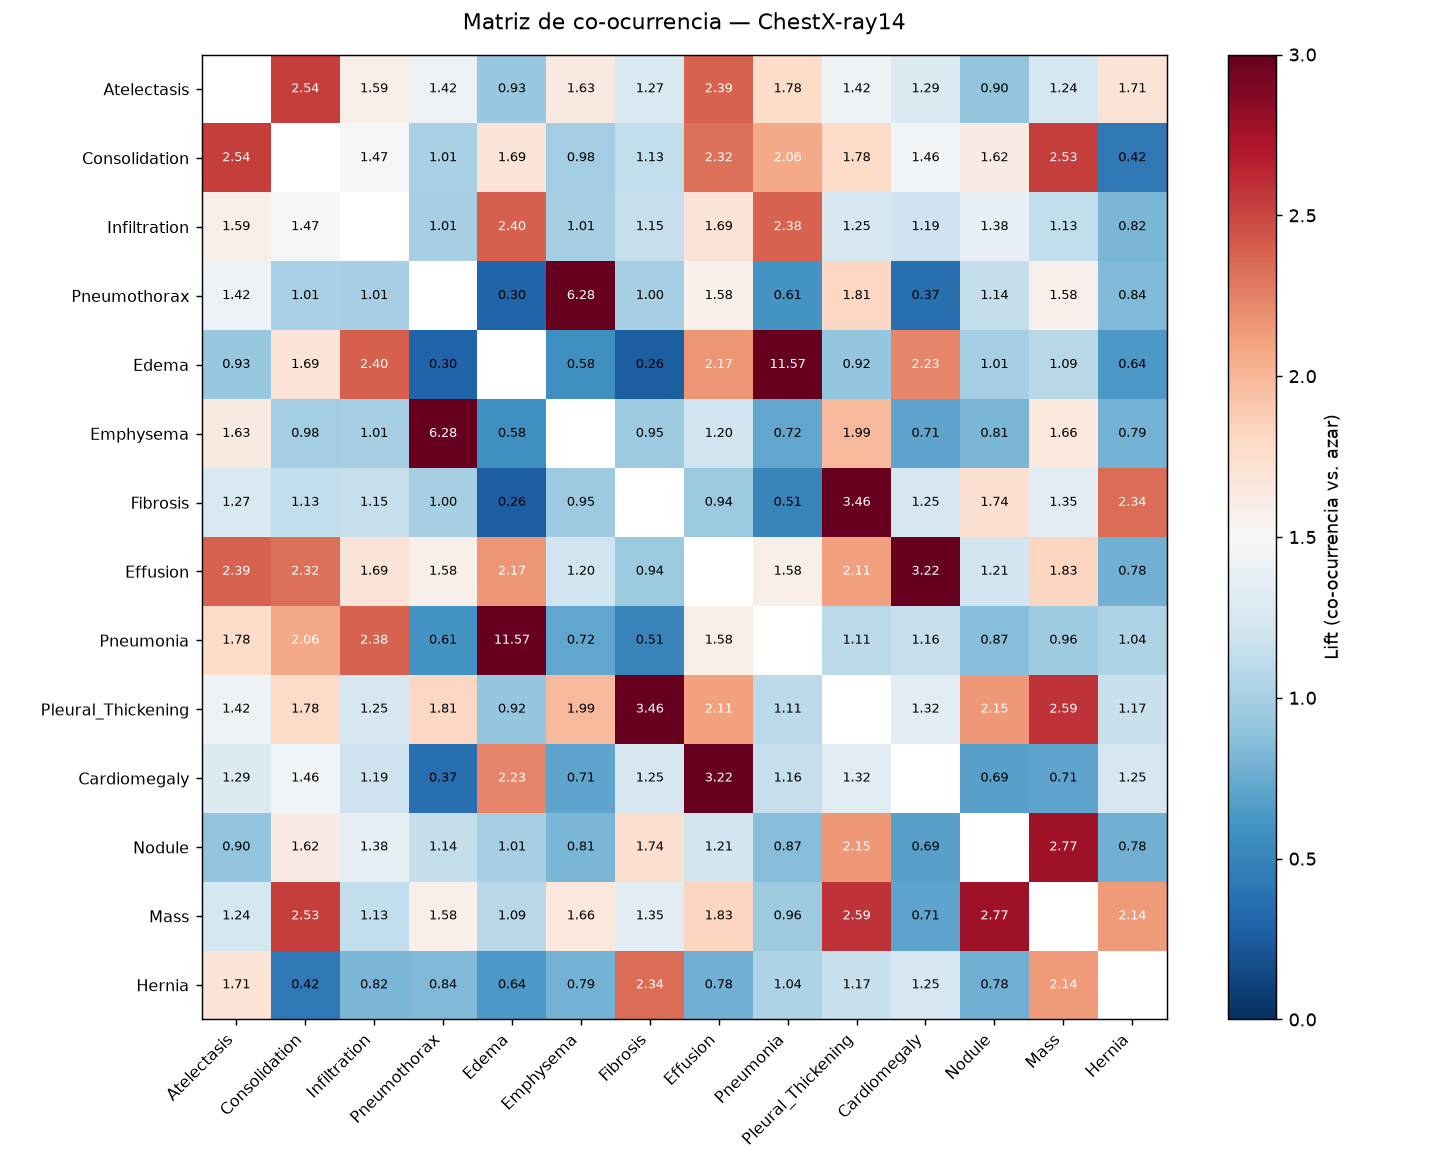
\includegraphics[width=0.66\linewidth]{co_ocurrencia.png}
    \caption{Matriz de co-ocurrencia (lift) entre las 14 patologías}
    \label{fig:coocurrencia}
\end{figure}

\begin{table}[H]
\centering
\small
\caption{Pares de patologías con mayor lift}
\label{tab:lift}
\begin{tabularx}{\textwidth}{L{5cm} r r X}
\toprule
Par & Casos & Lift & Interpretación del reporte \\
\midrule
Edema + Pneumonia & 340 & 11,57 & Edema perilesional y complicación aspirativa de la neumonía \\
Pneumothorax + Emphysema & 747 & 6,28 & Rotura de bullas enfisematosas y neumotórax espontáneo \\
Fibrosis + Pleural\_Thickening & 176 & 3,46 & Fibrosis subpleural con engrosamiento pleural periférico \\
Effusion + Cardiomegaly & 1.063 & 3,22 & Insuficiencia cardíaca congestiva \\
Nodule + Mass & 906 & 2,78 & Espectro continuo: un nódulo es una masa menor a 3 cm \\
\bottomrule
\end{tabularx}
\end{table}

Estas interpretaciones son hipótesis generadas para el reporte y no han sido validadas por un profesional de la salud. Los pares con clases poco frecuentes deben leerse con cautela.

\subsection{División por paciente}

\begin{table}[H]
\centering
\small
\caption{Resultado de la división del dataset}
\label{tab:split}
\begin{tabular}{l r r r r}
\toprule
Conjunto & Imágenes & \% imágenes & Pacientes & \% pacientes \\
\midrule
Entrenamiento & 76.277 & 68,03\% & 24.647 & 80,01\% \\
Validación & 10.247 & 9,14\% & 3.361 & 10,91\% \\
Prueba & 25.596 & 22,83\% & 2.797 & 9,08\% \\
\midrule
\textbf{Total} & \textbf{112.120} & \textbf{100\%} & \textbf{30.805} & \textbf{100\%} \\
\bottomrule
\end{tabular}
\end{table}

La suma de pacientes por conjunto coincide con el total de pacientes únicos, lo que es consistente con la verificación que hace el script: ningún paciente se repite entre conjuntos.

\subsection{Pesos por clase}

\begin{table}[H]
\centering
\small
\caption{Frecuencia y peso por clase en el conjunto de entrenamiento}
\label{tab:pesos}
\begin{tabular}{l r r r}
\toprule
Patología & Positivos & Frecuencia & Peso (raíz) \\
\midrule
Atelectasis & 7.236 & 9,49\% & 3,09 \\
Consolidation & 2.542 & 3,33\% & 5,39 \\
Infiltration & 12.190 & 15,98\% & 2,29 \\
Pneumothorax & 2.337 & 3,06\% & 5,62 \\
Edema & 1.234 & 1,62\% & 7,80 \\
Emphysema & 1.295 & 1,70\% & 7,61 \\
Fibrosis & 1.084 & 1,42\% & 8,33 \\
Effusion & 7.638 & 10,01\% & 3,00 \\
Pneumonia & 765 & 1,00\% & 9,94 \\
Pleural\_Thickening & 1.931 & 2,53\% & 6,20 \\
Cardiomegaly & 1.509 & 1,98\% & 7,04 \\
Nodule & 4.146 & 5,44\% & 4,17 \\
Mass & 3.554 & 4,66\% & 4,52 \\
Hernia & 115 & 0,15\% & 25,73 \\
\bottomrule
\end{tabular}
\end{table}

\subsection{Entrenamiento de prueba}

El modelo actual se entrenó con el subconjunto de 2.000 imágenes durante 2 épocas, solo para comprobar que el flujo de entrenamiento funciona.

\begin{table}[H]
\centering
\small
\caption{Métricas del entrenamiento de prueba (\texttt{log\_etapa1.csv})}
\label{tab:sanity}
\begin{tabular}{c r r r r}
\toprule
Época & AUC entrenamiento & Pérdida entrenamiento & AUC validación & Pérdida validación \\
\midrule
1 & 0,529 & 0,905 & 0,565 & 0,573 \\
2 & 0,564 & 0,852 & 0,611 & 0,545 \\
\bottomrule
\end{tabular}
\end{table}

Las métricas mejoran entre ambas épocas, lo que indica que el flujo de entrenamiento aprende. Con 2 épocas y un subconjunto, el valor de 0,61 \textbf{no es comparable con la literatura} y no sirve para evaluar RNF8. Tampoco se dispone aún de curvas de aprendizaje ni de métricas en el conjunto de prueba.

% ==========================================================
\section{Arquitectura implementada}
% ==========================================================

\subsection{Diagrama de arquitectura}

Se mantiene el flujo definido en el Hito 1: GUI $\rightarrow$ DCM $\rightarrow$ PRE $\rightarrow$ CLS $\rightarrow$ LOC $\rightarrow$ GUI. En desarrollo, TRN usa PRE para entrenar a CLS y entrega los pesos del modelo.

\begin{figure}[H]
\centering
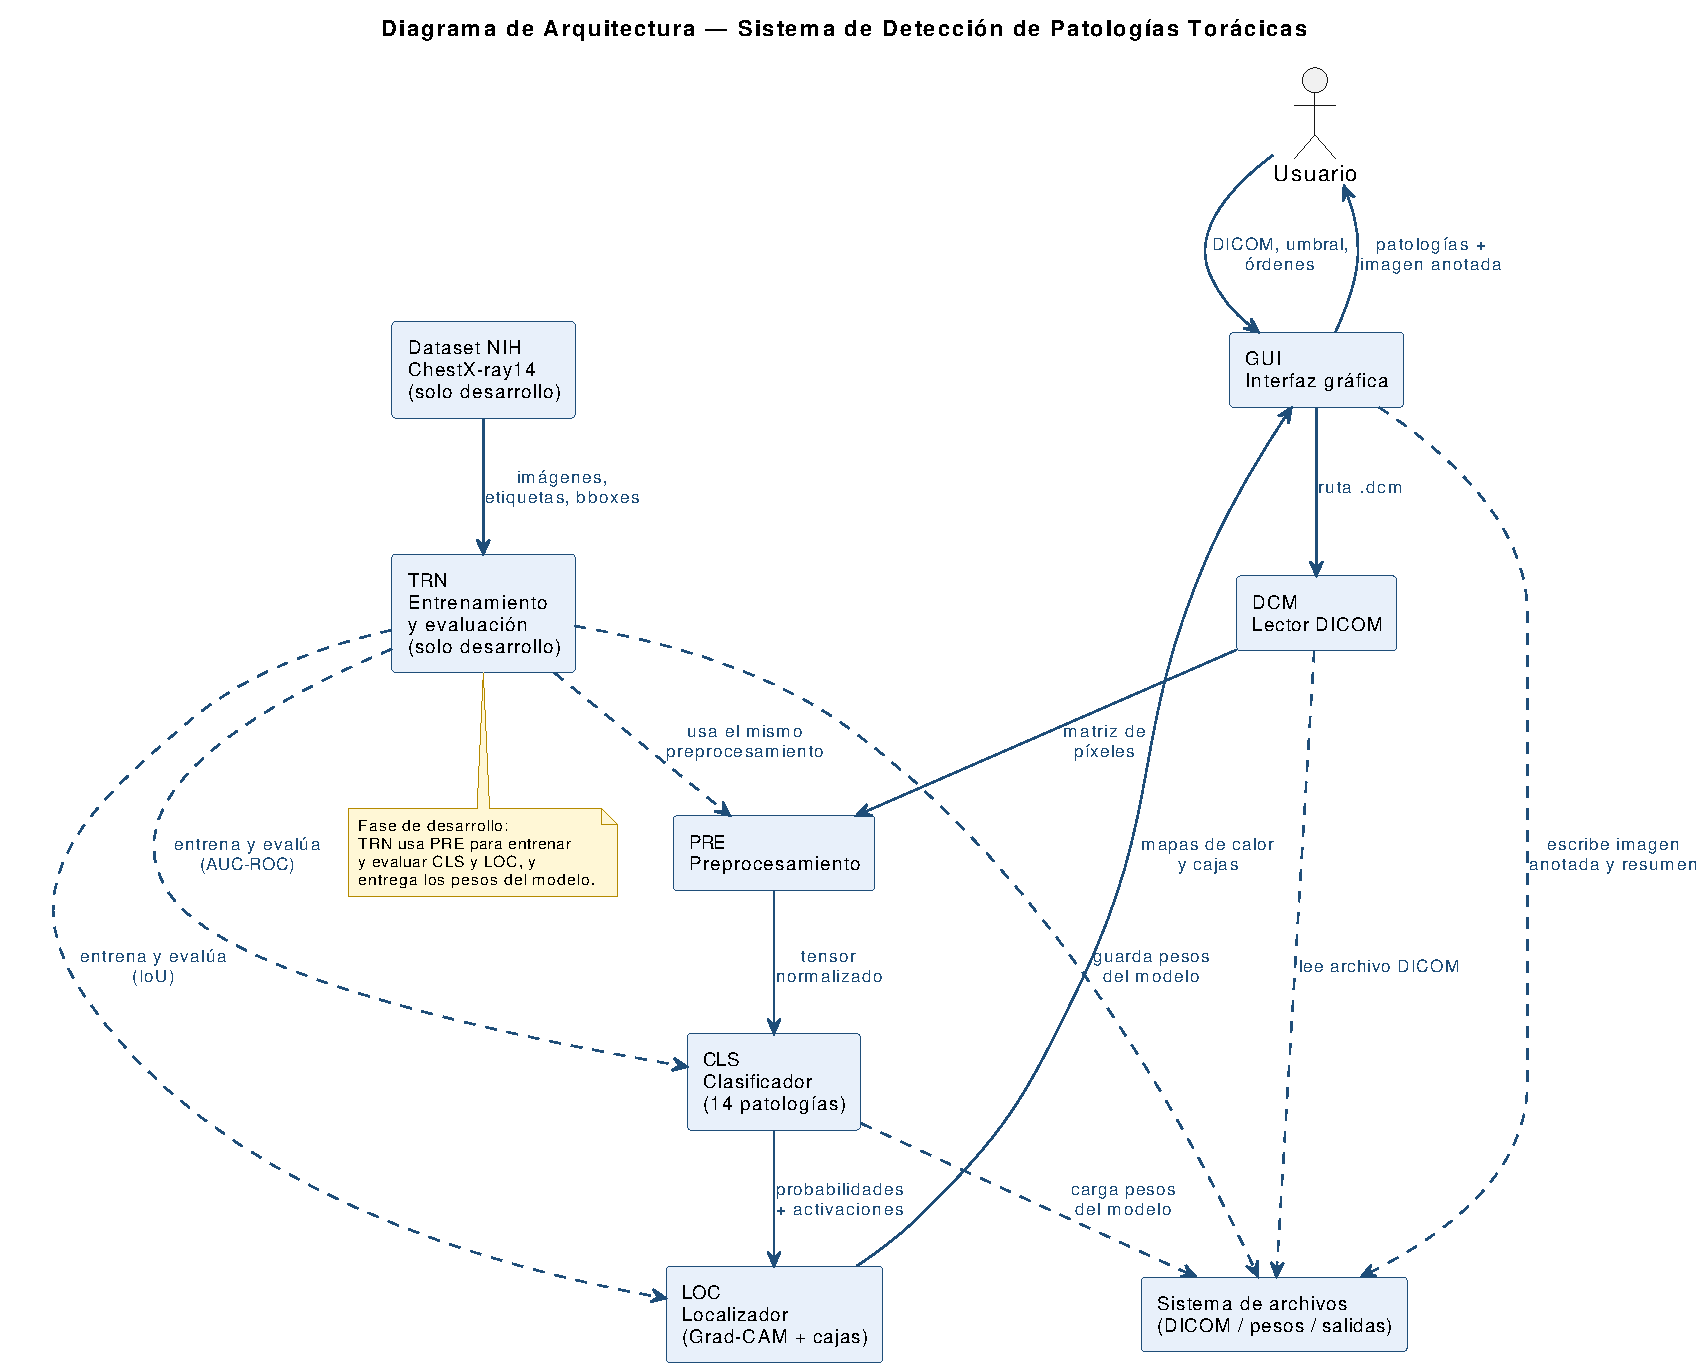
\includegraphics[width=0.66\textwidth]{Diagrama de Arquitectura.pdf}
\caption{Diagrama de arquitectura del sistema}
\label{fig:arquitectura}
\end{figure}

\subsection{Módulos y código}

\begin{table}[H]
\centering
\small
\caption{Implementación de los módulos}
\label{tab:modulos}
\begin{tabularx}{\textwidth}{L{3.6cm} L{4.2cm} X}
\toprule
Módulo & Archivo & Funciones principales \\
\midrule
Lector DICOM (DCM) & \texttt{06\_gui.py} & \texttt{load\_dicom}, \texttt{load\_png}, \texttt{cargar\_imagen} \\
Preprocesamiento (PRE) & \texttt{05\_entrenar.py}, \texttt{06\_gui.py} & \texttt{to\_224\_rgb}, \texttt{normalize}, \texttt{\_preprocess\_real} \\
Clasificador (CLS) & \texttt{05\_entrenar.py}, \texttt{06\_gui.py} & \texttt{build\_model}, \texttt{predict} \\
Localizador (LOC) & \texttt{06\_gui.py} & \texttt{heatmap}, \texttt{to\_boxes} \\
Interfaz gráfica (GUI) & \texttt{06\_gui.py} & \texttt{construir} y funciones \texttt{on\_*} \\
Entrenamiento y evaluación (TRN) & \texttt{01} a \texttt{05} & Preparación de datos y entrenamiento. La evaluación en prueba está pendiente \\
\bottomrule
\end{tabularx}
\end{table}

\subsection{Cambios respecto del diseño del Hito 1}

\begin{table}[H]
\centering
\small
\caption{Decisiones tomadas durante la implementación}
\label{tab:cambios}
\begin{tabularx}{\textwidth}{L{3.2cm} X X}
\toprule
Aspecto & Diseño del Hito 1 & Implementación \\
\midrule
Framework del modelo & PyTorch o TensorFlow/Keras & TensorFlow/Keras \\
Interfaz & PyQt, Tkinter, Streamlit o Gradio & Gradio, servida localmente en \texttt{127.0.0.1} \\
Tamaño de entrada & 224$\times$224 o 320$\times$320 & 224$\times$224 \\
Estructura del código & Una clase por módulo & Funciones agrupadas por script \\
Preprocesamiento & Módulo único & La misma lógica está duplicada en \texttt{05\_entrenar.py} y \texttt{06\_gui.py} \\
Formatos de entrada & DICOM & DICOM y PNG \\
Exportación & Diálogo de guardado & Carpeta automática \texttt{resultados/} con PNG, CSV y JSON, descargables desde la aplicación \\
Umbral inicial & 0,50 en el prototipo & 0,30, con rango de 0,05 a 0,95 \\
\bottomrule
\end{tabularx}
\end{table}

\subsection{Estado de los requisitos}

\begin{table}[H]
\centering
\footnotesize
\caption{Estado de los requisitos en el corte de la semana 14}
\label{tab:requisitos}
\begin{tabularx}{\textwidth}{L{4.1cm} L{1.9cm} X}
\toprule
Requisito & Estado & Observación \\
\midrule
\filaC RF1 Cargar imagen DICOM & Implementado & También acepta PNG \\
\filaP RF2 Validar archivo & Parcial & Valida que sea DICOM, en escala de grises y 2D. No comprueba que sea una radiografía de tórax \\
\filaC RF3 Visualizar imagen & Implementado & Visor de la pantalla principal \\
\filaC RF4 Preprocesar imagen & Implementado & Aplica escala, ventana, inversión de MONOCHROME1 y redimensionamiento \\
\filaC RF5 Detectar patologías & Implementado & Entrega 14 probabilidades con el modelo de prueba \\
\filaP RF6 Localizar patologías & Parcial & Grad-CAM y cajas funcionan. Falta evaluar su calidad con IoU \\
\filaC RF7 Mostrar resultados & Implementado & Lista, barras, cajas y mapa de calor \\
\filaC RF8 Ajustar umbral & Implementado & Al soltar el control se repite el análisis completo \\
\filaC RF9 Exportar resultados & Implementado & Imagen anotada, CSV y JSON \\
\filaP RF10 Entrenar y evaluar & Parcial & Entrenamiento implementado. Falta el entrenamiento completo y la evaluación en prueba \\
\midrule
RNF1 Rendimiento & Sin medir & Depende de la prueba PS1 \\
\filaP RNF2 Usabilidad & Parcial & El flujo es cargar, analizar y ver resultados. Falta la prueba con usuarios (PS5) \\
\filaP RNF3 Portabilidad & Parcial & Solo hay evidencia de ejecución en Linux \\
\filaP RNF4 Mantenibilidad & Parcial & Código documentado y versionado, con lógica de preprocesamiento duplicada \\
\filaC RNF5 Privacidad y seguridad & Implementado & Ejecución local. Solo se escriben archivos cuando el usuario exporta \\
\filaP RNF6 Reproducibilidad & Parcial & Hay semillas en división, subconjunto y mezcla, pero no una semilla global para el entrenamiento \\
\filaP RNF7 Transparencia & Parcial & El aviso está en la barra de estado, pero en la grabación queda bajo el borde visible de la ventana \\
RNF8 Desempeño del modelo & Pendiente & Requiere el entrenamiento completo y PM2 \\
\bottomrule
\end{tabularx}
\end{table}

% ==========================================================
\section{Interfaz implementada}
% ==========================================================

La aplicación sigue la distribución del Prototipo 1 del Hito 1: visor a la izquierda, panel de resultados a la derecha y controles en la parte inferior. Las figuras son cuadros del video de demostración, grabado el 5 de noviembre de 2026 con el modelo de prueba. Sus valores solo ilustran el funcionamiento y no tienen validez clínica.

\begin{figure}[H]
    \centering
    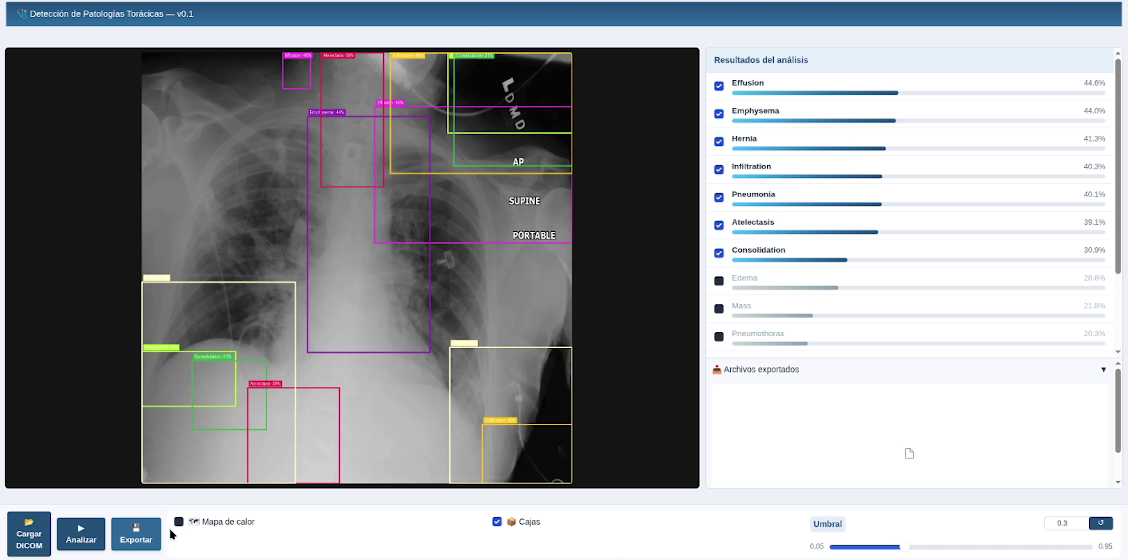
\includegraphics[width=0.7\linewidth]{gui_cajas.png}
    \caption{Resultado del análisis con cajas y umbral 0,30}
    \label{fig:guicajas}
\end{figure}

\begin{figure}[H]
    \centering
    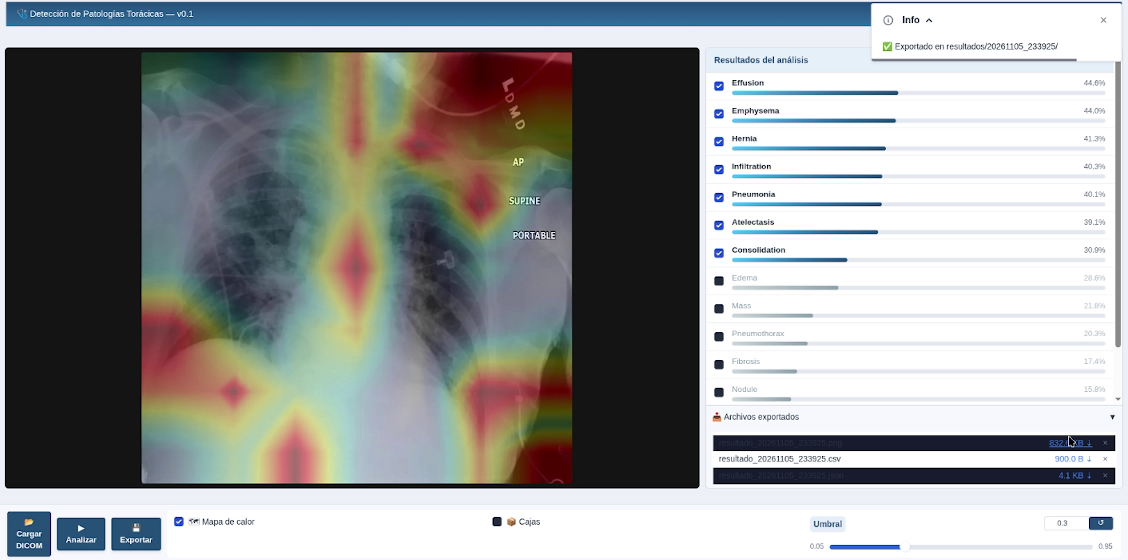
\includegraphics[width=0.7\linewidth]{gui_mapa.png}
    \caption{Mapa de calor de Grad-CAM y archivos exportados}
    \label{fig:guimapa}
\end{figure}

\begin{figure}[H]
    \centering
    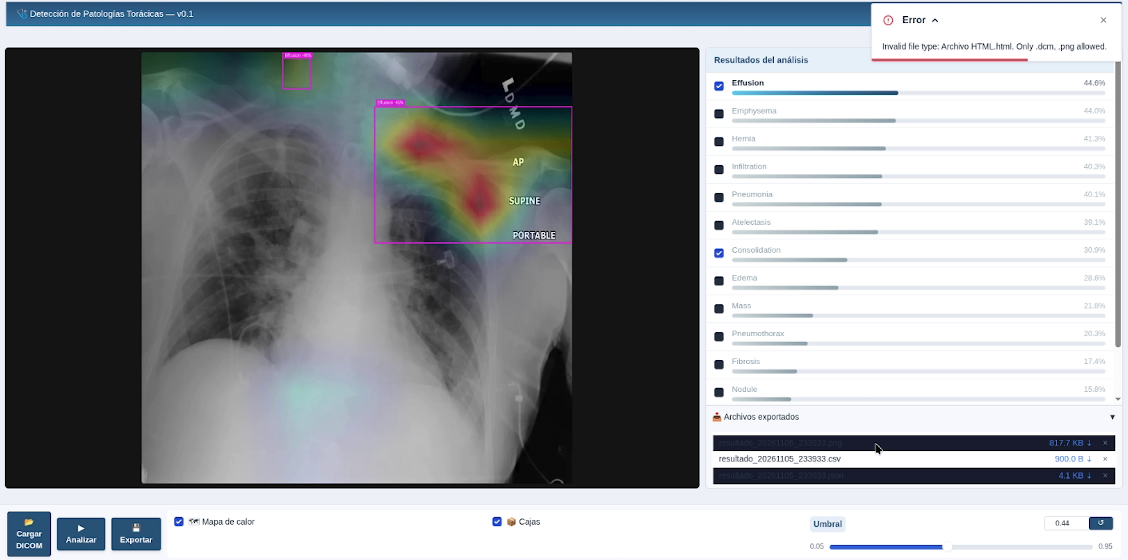
\includegraphics[width=0.7\linewidth]{gui_umbral.png}
    \caption{Selección de patologías, cambio de umbral y rechazo de un archivo no permitido}
    \label{fig:guiumbral}
\end{figure}

\begin{figure}[H]
    \centering
    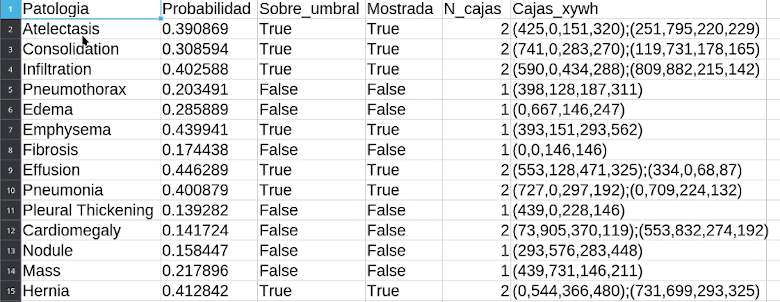
\includegraphics[width=0.62\linewidth]{gui_csv.png}
    \caption{Resumen exportado en CSV}
    \label{fig:guicsv}
\end{figure}

\begin{figure}[H]
    \centering
    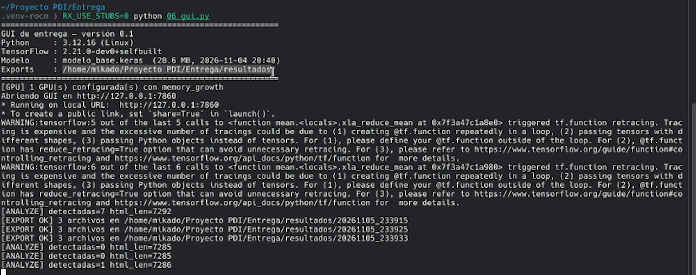
\includegraphics[width=0.75\linewidth]{gui_consola.png}
    \caption{Consola de la demostración: modelo real (\texttt{RX\_USE\_STUBS=0})}
    \label{fig:guiconsola}
\end{figure}

\begin{table}[H]
\centering
\small
\caption{Interacciones implementadas}
\label{tab:interacciones}
\begin{tabularx}{\textwidth}{L{3cm} X L{5cm}}
\toprule
Evento & Acción & Objeto afectado \\
\midrule
Cargar DICOM & Carga y valida el archivo. Si es válido, muestra la imagen & Visor, barra de estado \\
Analizar & Ejecuta el modelo y Grad-CAM para las 14 patologías & Visor, panel de resultados \\
Cambiar umbral & Repite el análisis y marca las patologías sobre el umbral & Visor, panel de resultados \\
Marcar patología & Muestra u oculta su región & Visor \\
Mapa de calor / Cajas & Activa o desactiva cada capa sobre la imagen & Visor \\
Exportar & Guarda imagen anotada, CSV y JSON y permite descargarlos & Archivos exportados \\
Archivo inválido & Muestra un mensaje de error emergente y no ejecuta el análisis & Notificación \\
\bottomrule
\end{tabularx}
\end{table}

\textbf{Observación de la demostración.} Las probabilidades son parecidas entre sí y varias regiones caen sobre marcadores de la placa o fuera del pulmón. Esto es esperable en un modelo de prueba y confirma que la localización todavía no puede considerarse confiable. Su calidad se medirá con la prueba PM3 sobre el modelo completo.

% ==========================================================
\section{Pruebas}
\label{sec:pruebas}
% ==========================================================

\subsection{Pruebas automatizadas}

El reporte generado el 6 de noviembre de 2026 registra \textbf{26 pruebas aprobadas de 26}, sin fallas, en 24,12 segundos. La ejecución excluye por diseño la prueba \texttt{test\_pu5\_heatmap\_forma}, marcada como dependiente del modelo. Las pruebas usan principalmente datos sintéticos, y las de CLS verifican la arquitectura sin pesos entrenados.

\begin{table}[H]
\centering
\small
\caption{Resultado de las pruebas automatizadas por archivo}
\label{tab:tests}
\begin{tabularx}{\textwidth}{L{3cm} r r X}
\toprule
Archivo & Total & Aprobadas & Qué verifica \\
\midrule
\texttt{test\_dcm} & 6 & 6 & Lectura de DICOM, inversión, ventana, percentiles y rechazo de archivos inválidos \\
\texttt{test\_loc} & 3 & 3 & Cajas dentro de los límites, mapa vacío y escala \\
\texttt{test\_model} & 3 & 3 & Salida de 14 valores entre 0 y 1, capa de Grad-CAM y compilación \\
\texttt{test\_pre} & 3 & 3 & Forma, tipo y normalización de la imagen \\
\texttt{test\_split} & 4 & 4 & Sin pacientes repetidos, orden de columnas y proporción de validación \\
\texttt{test\_subset} & 2 & 2 & Subconjunto con todas las clases y positivos mínimos \\
\texttt{test\_verify} & 2 & 2 & Conteos y codificación multi-etiqueta \\
\texttt{test\_weights} & 3 & 3 & Catorce pesos positivos, con Hernia como el mayor \\
\midrule
\textbf{Total} & \textbf{26} & \textbf{26} & \\
\bottomrule
\end{tabularx}
\end{table}

\subsection{Estado del plan de pruebas}

\begin{table}[H]
\centering
\footnotesize
\caption{Avance del plan de pruebas del Hito 1}
\label{tab:plan}
\begin{tabularx}{\textwidth}{L{0.9cm} X L{1.9cm} X}
\toprule
ID & Prueba & Estado & Evidencia u observación \\
\midrule
\filaC PM1 & Sin pacientes repetidos entre conjuntos & Aprobada & Verificación en \texttt{02\_split\_dataset.py}, \texttt{test\_split} y log de división \\
PM2 & AUC-ROC por patología en prueba & Pendiente & Requiere el entrenamiento completo \\
PM3 & IoU contra cajas reales & Pendiente & Requiere el modelo completo y un script de evaluación \\
PM4 & Reproducibilidad con la misma semilla & Pendiente & Falta fijar una semilla global de entrenamiento \\
\midrule
\filaC PU1 & DCM lee un DICOM válido & Aprobada & \texttt{test\_dcm}, con DICOM sintéticos \\
\filaC PU2 & DCM rechaza un archivo no DICOM & Aprobada & \texttt{test\_dcm} \\
\filaP PU3 & PRE equivalente para PNG y DICOM & Parcial & \texttt{test\_pre} y comparación con una imagen sintética de 8 bits. Falta comparar el flujo completo y DICOM de 12--16 bits \\
\filaC PU4 & CLS entrega 14 valores entre 0 y 1 & Aprobada & \texttt{test\_model}, sin pesos entrenados \\
\filaC PU5 & LOC entrega cajas dentro de la imagen & Aprobada & \texttt{test\_loc} \\
\midrule
\filaP PS1 & Flujo completo en menos de 10 s & Parcial & Flujo demostrado en video. Falta medir el tiempo \\
\filaP PS2 & Cambiar el umbral & Parcial & Demostrado en video. Falta la prueba formal \\
\filaP PS3 & Exportar resultados & Parcial & Demostrado en video. Falta la prueba formal \\
\filaP PS4 & Cargar un archivo inválido & Parcial & Demostrado en video con un archivo HTML. Faltan otros casos, como un DICOM dañado \\
PS5 & Usabilidad con usuarios objetivo & Pendiente & Planificada para la semana 17 \\
\bottomrule
\end{tabularx}
\end{table}

% ==========================================================
\section{Seguimiento y próximos pasos}
% ==========================================================

\subsection{Tareas del siguiente ciclo (semana 15)}

\begin{itemize}
    \item \textbf{Nicolas:} ejecutar el entrenamiento completo con 76.277 imágenes (3 + 10 épocas) y preparar las curvas de aprendizaje y la evaluación AUC-ROC.
    \item \textbf{Karime:} evaluar el IoU con \texttt{BBox\_List\_2017}.
    \item \textbf{Benjamin:} refinar la GUI.
    \item \textbf{Todo el equipo:} incorporar los comentarios del profesor sobre el documento del Hito 1 y mantener las reuniones semanales.
\end{itemize}

\subsection{Impedimentos y riesgos}

\begin{table}[H]
\centering
\small
\caption{Impedimentos y riesgos}
\label{tab:riesgos}
\begin{tabularx}{\textwidth}{X X}
\toprule
Impedimento o riesgo & Acción \\
\midrule
El entrenamiento completo requiere de 6 a 8 horas de GPU dedicada & Ejecutarlo en la semana 15, según lo asignado en la Bitácora 2 \\
Las evaluaciones de AUC e IoU dependen del modelo completo & Priorizar el entrenamiento antes de esas tareas \\
Congelamientos del sistema operativo bajo carga de GPU & Crecimiento gradual de VRAM y concurrencia limitada en la GUI \\
El método de localización podría ser insuficiente & Decidir con los resultados de IoU si Grad-CAM basta o se requiere un detector \\
Solo 8 de las 14 patologías tienen cajas reales & Informar el IoU solo para esas 8 patologías \\
\bottomrule
\end{tabularx}
\end{table}

\subsection{Próximos hitos}

\begin{itemize}
    \item \textbf{Milestone 3}, sistema integrado: semana 17 (del 23/11 al 27/11).
    \item \textbf{Milestone 4}, Feria y Bitácora 3: semana 18 (del 30/11 al 04/12).
\end{itemize}

% ==========================================================
\section{Conclusiones}
% ==========================================================

El Hito 2 convierte el diseño del Hito 1 en una cadena funcional: desde la verificación y división del dataset hasta una aplicación que lee DICOM, ejecuta el modelo, marca regiones y exporta resultados. Se comprobó la división sin pacientes repetidos, y las 26 pruebas automatizadas ejecutadas fueron aprobadas.

El principal pendiente es el desempeño. El modelo disponible es de prueba, por lo que todavía no se puede afirmar nada sobre la calidad de la clasificación ni de la localización. El siguiente ciclo se concentra en el entrenamiento completo y en las evaluaciones AUC-ROC e IoU, que permitirán fijar la meta de desempeño y decidir si Grad-CAM es suficiente.

% ==========================================================
\section{Referencias}
\label{sec:refs}
% ==========================================================

\begin{enumerate}
    \item X. Wang, Y. Peng, L. Lu, Z. Lu, M. Bagheri y R. M. Summers, ``ChestX-ray8: Hospital-scale chest X-ray database and benchmarks on weakly-supervised classification and localization of common thorax diseases,'' en \emph{Proc. IEEE CVPR}, 2017, pp. 3462--3471. (arXiv:1705.02315)
    \item P. Rajpurkar et al., ``CheXNet: Radiologist-level pneumonia detection on chest X-rays with deep learning,'' arXiv:1711.05225, 2017.
    \item R. R. Selvaraju et al., ``Grad-CAM: Visual explanations from deep networks via gradient-based localization,'' en \emph{Proc. IEEE ICCV}, 2017.
    \item G. Huang, Z. Liu, L. van der Maaten y K. Q. Weinberger, ``Densely connected convolutional networks,'' en \emph{Proc. IEEE CVPR}, 2017.
    \item M. Zúñiga, ``Elementos Iniciales de Planificación de Proyectos,'' material del curso, Departamento de Electrónica, Universidad Técnica Federico Santa María, septiembre de 2026.
\end{enumerate}

\appendix

% ==========================================================
\section{Guía de ejecución}
% ==========================================================

Los comandos se ejecutan desde la carpeta del código. Se necesita el dataset NIH ChestX-ray14 y, para la aplicación, el archivo \texttt{models/modelo\_base.keras}, que no forma parte de las evidencias.

\begin{lstlisting}[language=bash]
python 01_verificar_dataset.py --entry-csv /ruta/Data_Entry_2017.csv
python 02_split_dataset.py --dataset-dir /ruta/dataset
python 02-1_analisis_dataset.py --splits-dir data/splits --out-dir reportes
python 03_calcular_pesos.py --splits-dir data/splits
python 04_crear_subconjunto.py --splits-dir data/splits

# Entrenamiento de prueba
python 05_entrenar.py --images-dir /ruta/images --debug --epochs-head 3 --epochs-ft 0
# Entrenamiento completo
python 05_entrenar.py --images-dir /ruta/images --epochs-head 3 --epochs-ft 10

python 06_gui.py                # Aplicacion con el modelo entrenado
RX_USE_STUBS=1 python 06_gui.py # Aplicacion con datos simulados, sin modelo
python 11_reporte_test.py       # Pruebas y reporte
\end{lstlisting}

% ==========================================================
\section{Índice de evidencias}
\label{sec:evidencias}
% ==========================================================

\begin{table}[H]
\centering
\small
\caption{Evidencias del Hito 2 en la carpeta \texttt{evidencias/}}
\label{tab:evidencias}
\begin{tabularx}{\textwidth}{L{5.1cm} X}
\toprule
Ubicación & Contenido \\
\midrule
\texttt{codigo/} & Scripts del Cuadro~\ref{tab:scripts} y \texttt{pytest.ini} \\
\texttt{codigo/tests/} & Pruebas automatizadas \\
\texttt{logs/} & Salidas de verificación, división, entorno, pesos, consistencia, pruebas y entrenamiento \\
\texttt{capturas/} & Capturas de pantalla de cada tarea, identificadas con su ID \\
\texttt{reportes/} & Estadísticas, matrices de co-ocurrencia, gráficos y reporte de pruebas \\
\texttt{datos/} & Primeras filas de cada conjunto y \texttt{class\_weights.json} \\
\texttt{video/} & Demostración de la GUI (\texttt{Gui.mp4} y \texttt{Gui(1).mp4}) \\
\texttt{Copia de Bitacora\_2\_...xlsx} & Bitácora 2: tareas, Carta Gantt, seguimiento y calendario \\
\bottomrule
\end{tabularx}
\end{table}

\end{document}
